\section{Limits}
    \begin{frame}
		\frametitle{"Rough" Definition of a Limit}
		Suppose $f(x)$ is defined when $x$ is near the number $a$. (This means that $f$ is defined on some open interval that contains $a$, \alert{except possibly} at $a$ itself.)\\
		Then we write
		\begin{center}
			$\lim\limits_{\textit{x} \to a}f(x) = L$
		\end{center}
		and say
		\begin{center}
			"the limit if $f(x)$, as $x$ approaches $a$, equals $L$"
		\end{center}
		if we can make the values of $f(x)$ arbitrarily close to $L$ (as close to $L$ as we like) by taking $x$ to be \alert{sufficiently close to} $a$ (on either side of $a$) but \alert{not equal to} $a$.
	\end{frame}
	\begin{frame}
		\frametitle{One-sided Limits}
		Considering a function called \textit{Heaviside Function}\\
		\begin{center}
			\begin{equation}
				H(t)=
				\begin{cases}
					0 & t<0\\
					1 & t \geq 0
				\end{cases}
			\end{equation}
		\end{center}
		Does $\lim\limits_{\textit{t} \to 0}H(t)$ exists?
	\end{frame}
	\begin{frame}
		\frametitle{One-sided Limits}
		We write
		\begin{center}
			$\lim\limits_{\textit{x} \to a^{-}}f(x) = L$
		\end{center}
		and say the left-hand limit of $f(x)$ as $x$ approaches $a$ is equal to $L$ if we can make the values of $f(x)$ arbitrarily close to $L$ by taking $x$ to be \alert{sufficiently close to} $a$ and $x$ less than $a$.\\
		\bigskip
		When calculating $\lim\limits_{\textit{x} \to a^{-}}f(x)$, we consider only $x < a$.\\
		\bigskip
		Similarly, we can get the right-hand limit of $f(x)$ as $x$ approaches $a$.
	\end{frame}
	\begin{frame}
		\frametitle{One-sided Limits}
		When does $\lim\limits_{\textit{x} \to a}f(x)$ exists?\\
		\bigskip
		\begin{center}
			$\lim\limits_{\textit{x} \to a}f(x) = L$\\
			\bigskip
			\alert{if and only if}\\
			\bigskip
			$\lim\limits_{\textit{x} \to a^{-}}f(x) = L$ and $\lim\limits_{\textit{x} \to a^{+}}f(x) = L$
		\end{center}
		Can we directly regard $L$ as $f(a)$?
	\end{frame}
	\begin{frame}

		\frametitle{Infinite Limits}
		Let $f$ be a function defined on both sides of $a$, \alert{except possibly} at $a$ itself. Then
		\begin{center}
			$\lim\limits_{\textit{x} \to a}f(x) = \infty$
		\end{center}
		means that the values of $f(x)$ can be made arbitrarily large (as large as we please) by taking $x$ \alert{sufficiently close to} $a$, but \alert{not equal to} $a$.\\

		Let $f$ be a function defined on both sides of $a$, \alert{except possibly} at $a$ itself. Then
		\begin{center}
			$\lim\limits_{\textit{x} \to a}f(x) = -\infty$
		\end{center}
		means that the values of $f(x)$ can be made arbitrarily large negative by taking $x$ \alert{sufficiently close to} $a$, but \alert{not equal to} $a$.
	\end{frame}
	\begin{frame}
		\frametitle{Infinite Limits}
		\alert{Warning:}\\
		$\lim\limits_{\textit{x} \to a}f(x) = (-)\infty$ does not mean that we are regarding $(-)\infty$ as a number. Nor does it mean that the limit exists!
	\end{frame}
	\begin{frame}
		\frametitle{Limits at Infinity}
		\begin{enumerate}
			\item Let $f$ be a function defined on some interval ($a$, $\infty$). Then
			\begin{center}
				$\lim\limits_{\textit{x} \to \infty}f(x) = L$
			\end{center}
			means that the values of $f(x)$ can be made arbitrarily close to $L$ by taking $x$ sufficiently large.
		\item Let $f$ be a function defined on some interval ($-\infty$, $a$). Then
			\begin{center}
				$\lim\limits_{\textit{x} \to -\infty}f(x) = L$
			\end{center}
			means that the values of $f(x)$ can be made arbitrarily close to $L$ by taking $x$ sufficiently large negative.
		\end{enumerate}
	\end{frame}
	\begin{frame}
		\frametitle{Infinite Limits at Infinity}
		\begin{enumerate}
			\item $\lim\limits_{\textit{x} \to \infty}f(x) = \infty$
			\item $\lim\limits_{\textit{x} \to \infty}f(x) = -\infty$
			\item $\lim\limits_{\textit{x} \to -\infty}f(x) = \infty$
			\item $\lim\limits_{\textit{x} \to -\infty}f(x) = -\infty$
		\end{enumerate}
	\end{frame}
	\begin{frame}
		\frametitle{The Limit Laws}
		Five basic laws:\\
		Suppose that $c$ is a constant and the limits
		\begin{center}
			$\lim\limits_{\textit{x} \to a}f(x)$ and $\lim\limits_{\textit{x} \to a}g(x)$
		\end{center}
		exists. Then
		\begin{enumerate}
			\item $\lim\limits_{\textit{x} \to a}[f(x)+g(x)] = \lim\limits_{\textit{x} \to a}f(x) + \lim\limits_{\textit{x} \to a}g(x)$
			\item $\lim\limits_{\textit{x} \to a}[f(x)-g(x)] = \lim\limits_{\textit{x} \to a}f(x) - \lim\limits_{\textit{x} \to a}g(x)$
			\item $\lim\limits_{\textit{x} \to a}[cf(x)] = c\lim\limits_{\textit{x} \to a}f(x)$
			\item $\lim\limits_{\textit{x} \to a}[f(x)g(x)] = \lim\limits_{\textit{x} \to a}f(x) \cdot \lim\limits_{\textit{x} \to a}g(x)$
			\item $\lim\limits_{\textit{x} \to a}\dfrac{f(x)}{g(x)} = \dfrac{\lim\limits_{\textit{x} \to a}f(x)}{\lim\limits_{\textit{x} \to a}g(x)}$\ \ \  \alert{(if $\lim\limits_{\textit{x} \to a}g(x) \neq 0$)}
		\end{enumerate}
	\end{frame}
	\begin{frame}
		\frametitle{The Limit Laws}
		Another six laws:
		\begin{enumerate}
			\item $\lim\limits_{\textit{x} \to a}[f(x)]^{n} = [\lim\limits_{\textit{x} \to a}f(x)]^{n}$ (where $n$ is a positive integer)
			\item $\lim\limits_{\textit{x} \to a}c = c$
			\item $\lim\limits_{\textit{x} \to a}x = a$
			\item $\lim\limits_{\textit{x} \to a}x^{n} = a^{n}$ (where $n$ is a positive integer)
			\item $\lim\limits_{\textit{x} \to a}\sqrt[n]{x} = \sqrt[n]{a}$ (where $n$ is a positive integer)\\
				\alert{if $n$ is even, we assume that $a > 0$}
			\item $\lim\limits_{\textit{x} \to a}\sqrt[n]{f(x)} = \sqrt[n]{\lim\limits_{\textit{x} \to a}f(x)}$ (where $n$ is a positive integer)\\
				\alert{if $n$ is even, we assume that $\lim\limits_{\textit{x} \to a}f(x) > 0$}
		\end{enumerate} 
	\end{frame}
	\begin{frame}
		\frametitle{The Limit Laws}
		\alert{Warning:}\\
		The Limit Laws can't be applied to infinite limits because $(-)\infty$ is not a number!
	\end{frame}
	\begin{frame}
		\frametitle{The Limit Laws}
		Two additional properties of limits:
		\begin{enumerate}
				\item if $f(x) \leq g(x)$ when $x$ is near $a$ (\alert{except possibly} at $a$) and the limits of $f$ and $g$ both exists as $x$ approaches $a$, then
					\begin{center}
						$\lim\limits_{\textit{x} \to a}f(x) \leq \lim\limits_{\textit{x} \to a}g(x)$
					\end{center}
				\item \alert{(The Squeeze Theorem)} if $f(x) \leq g(x) \leq h(x)$ when $x$ is near $a$ (\alert{except possibly} at $a$) and
					\begin{center}
						$\lim\limits_{\textit{x} \to a}f(x) = \lim\limits_{\textit{x} \to a}h(x) = L$
					\end{center}
					then
					\begin{center}
						$\lim\limits_{\textit{x} \to a}g(x) = L$
					\end{center}
		\end{enumerate}
	\end{frame}

	\begin{frame}
		\frametitle{Two Important Limits}
		Be sure to keep these two limits in mind!
		\begin{enumerate}
			\item $\lim\limits_{\textit{x} \to 0}\dfrac{\sin{x}}{x} = 1$\\
				(How to prove it? Considering $\sin{x}$, $x$ and $\tan{x}$. Then, use the squeeze theorem.)
			\item $\lim\limits_{\textit{x} \to \infty}(1 + \dfrac{1}{x})^{x} = e = 2.718281828459045\cdots$
		\end{enumerate}
		\begin{columns}[c] % The "c" option specifies centered vertical alignment while the "t" option is used for top vertical alignment
			\begin{column}{0.5\textwidth} % Left column width
				\begin{figure}
					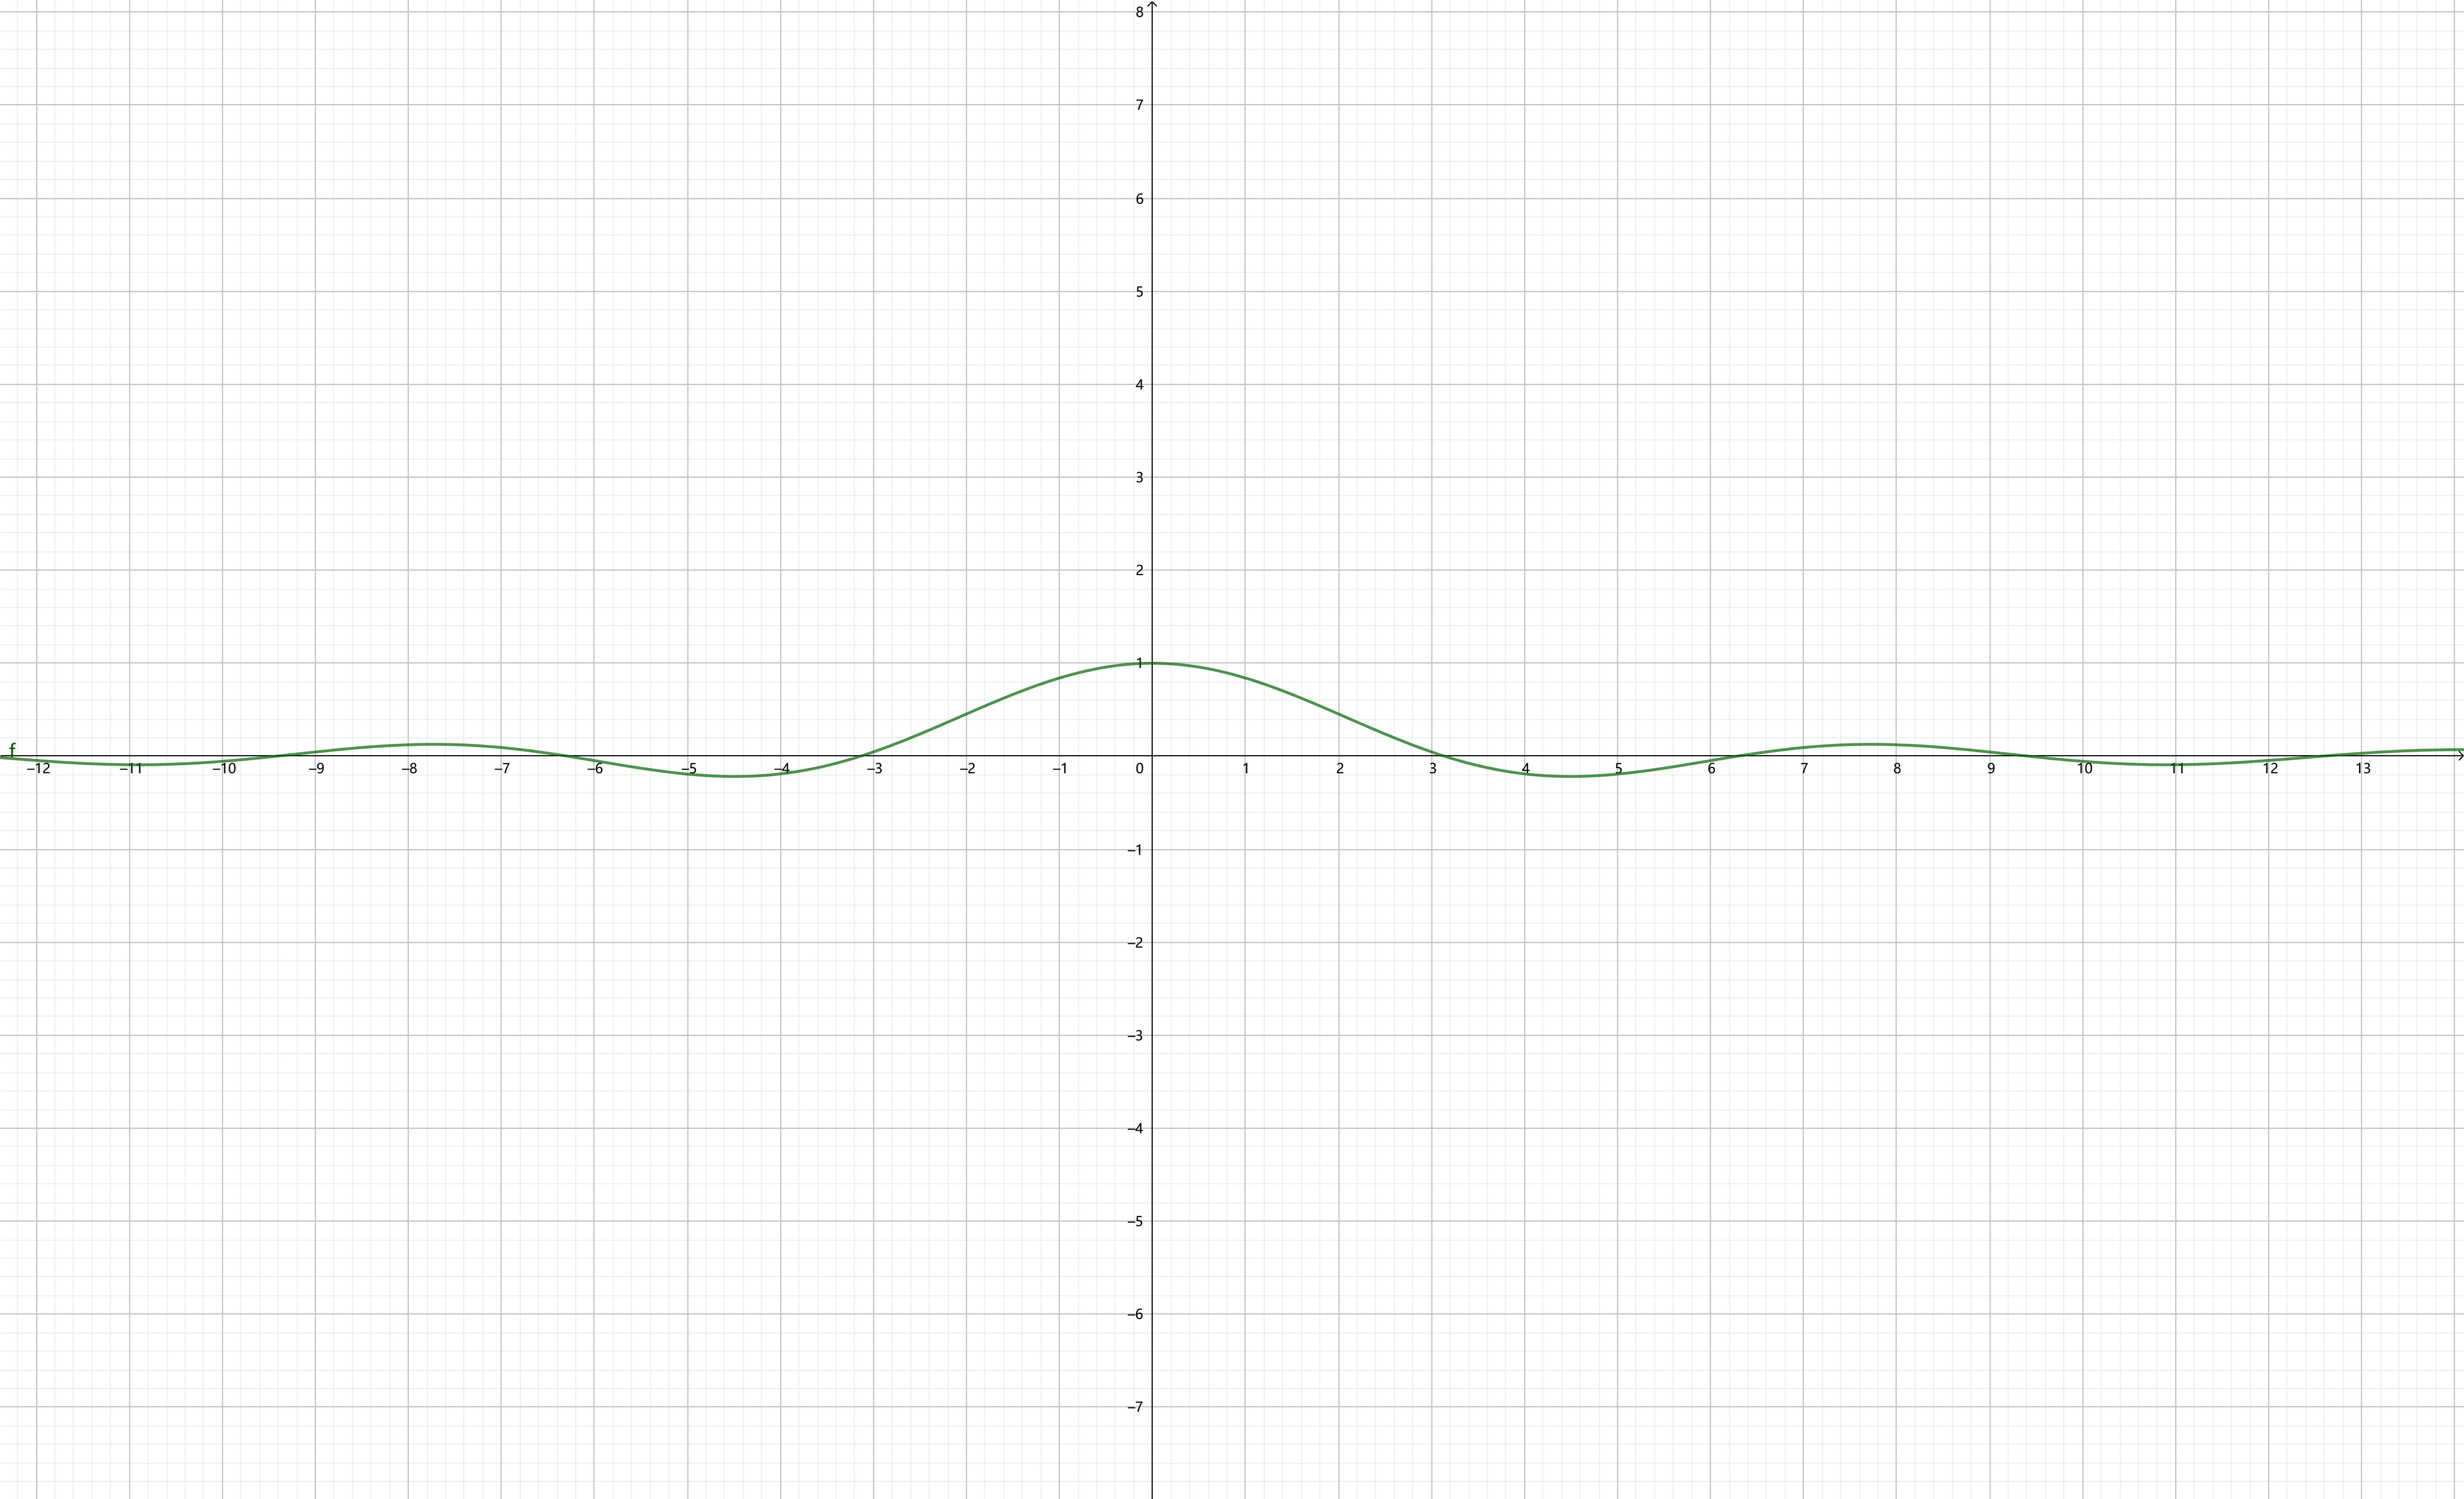
\includegraphics[width=1\linewidth]{res/bbb.jpg}
				\end{figure}
			\end{column}
			\begin{column}{0.5\textwidth} % Right column width
				\begin{figure}
					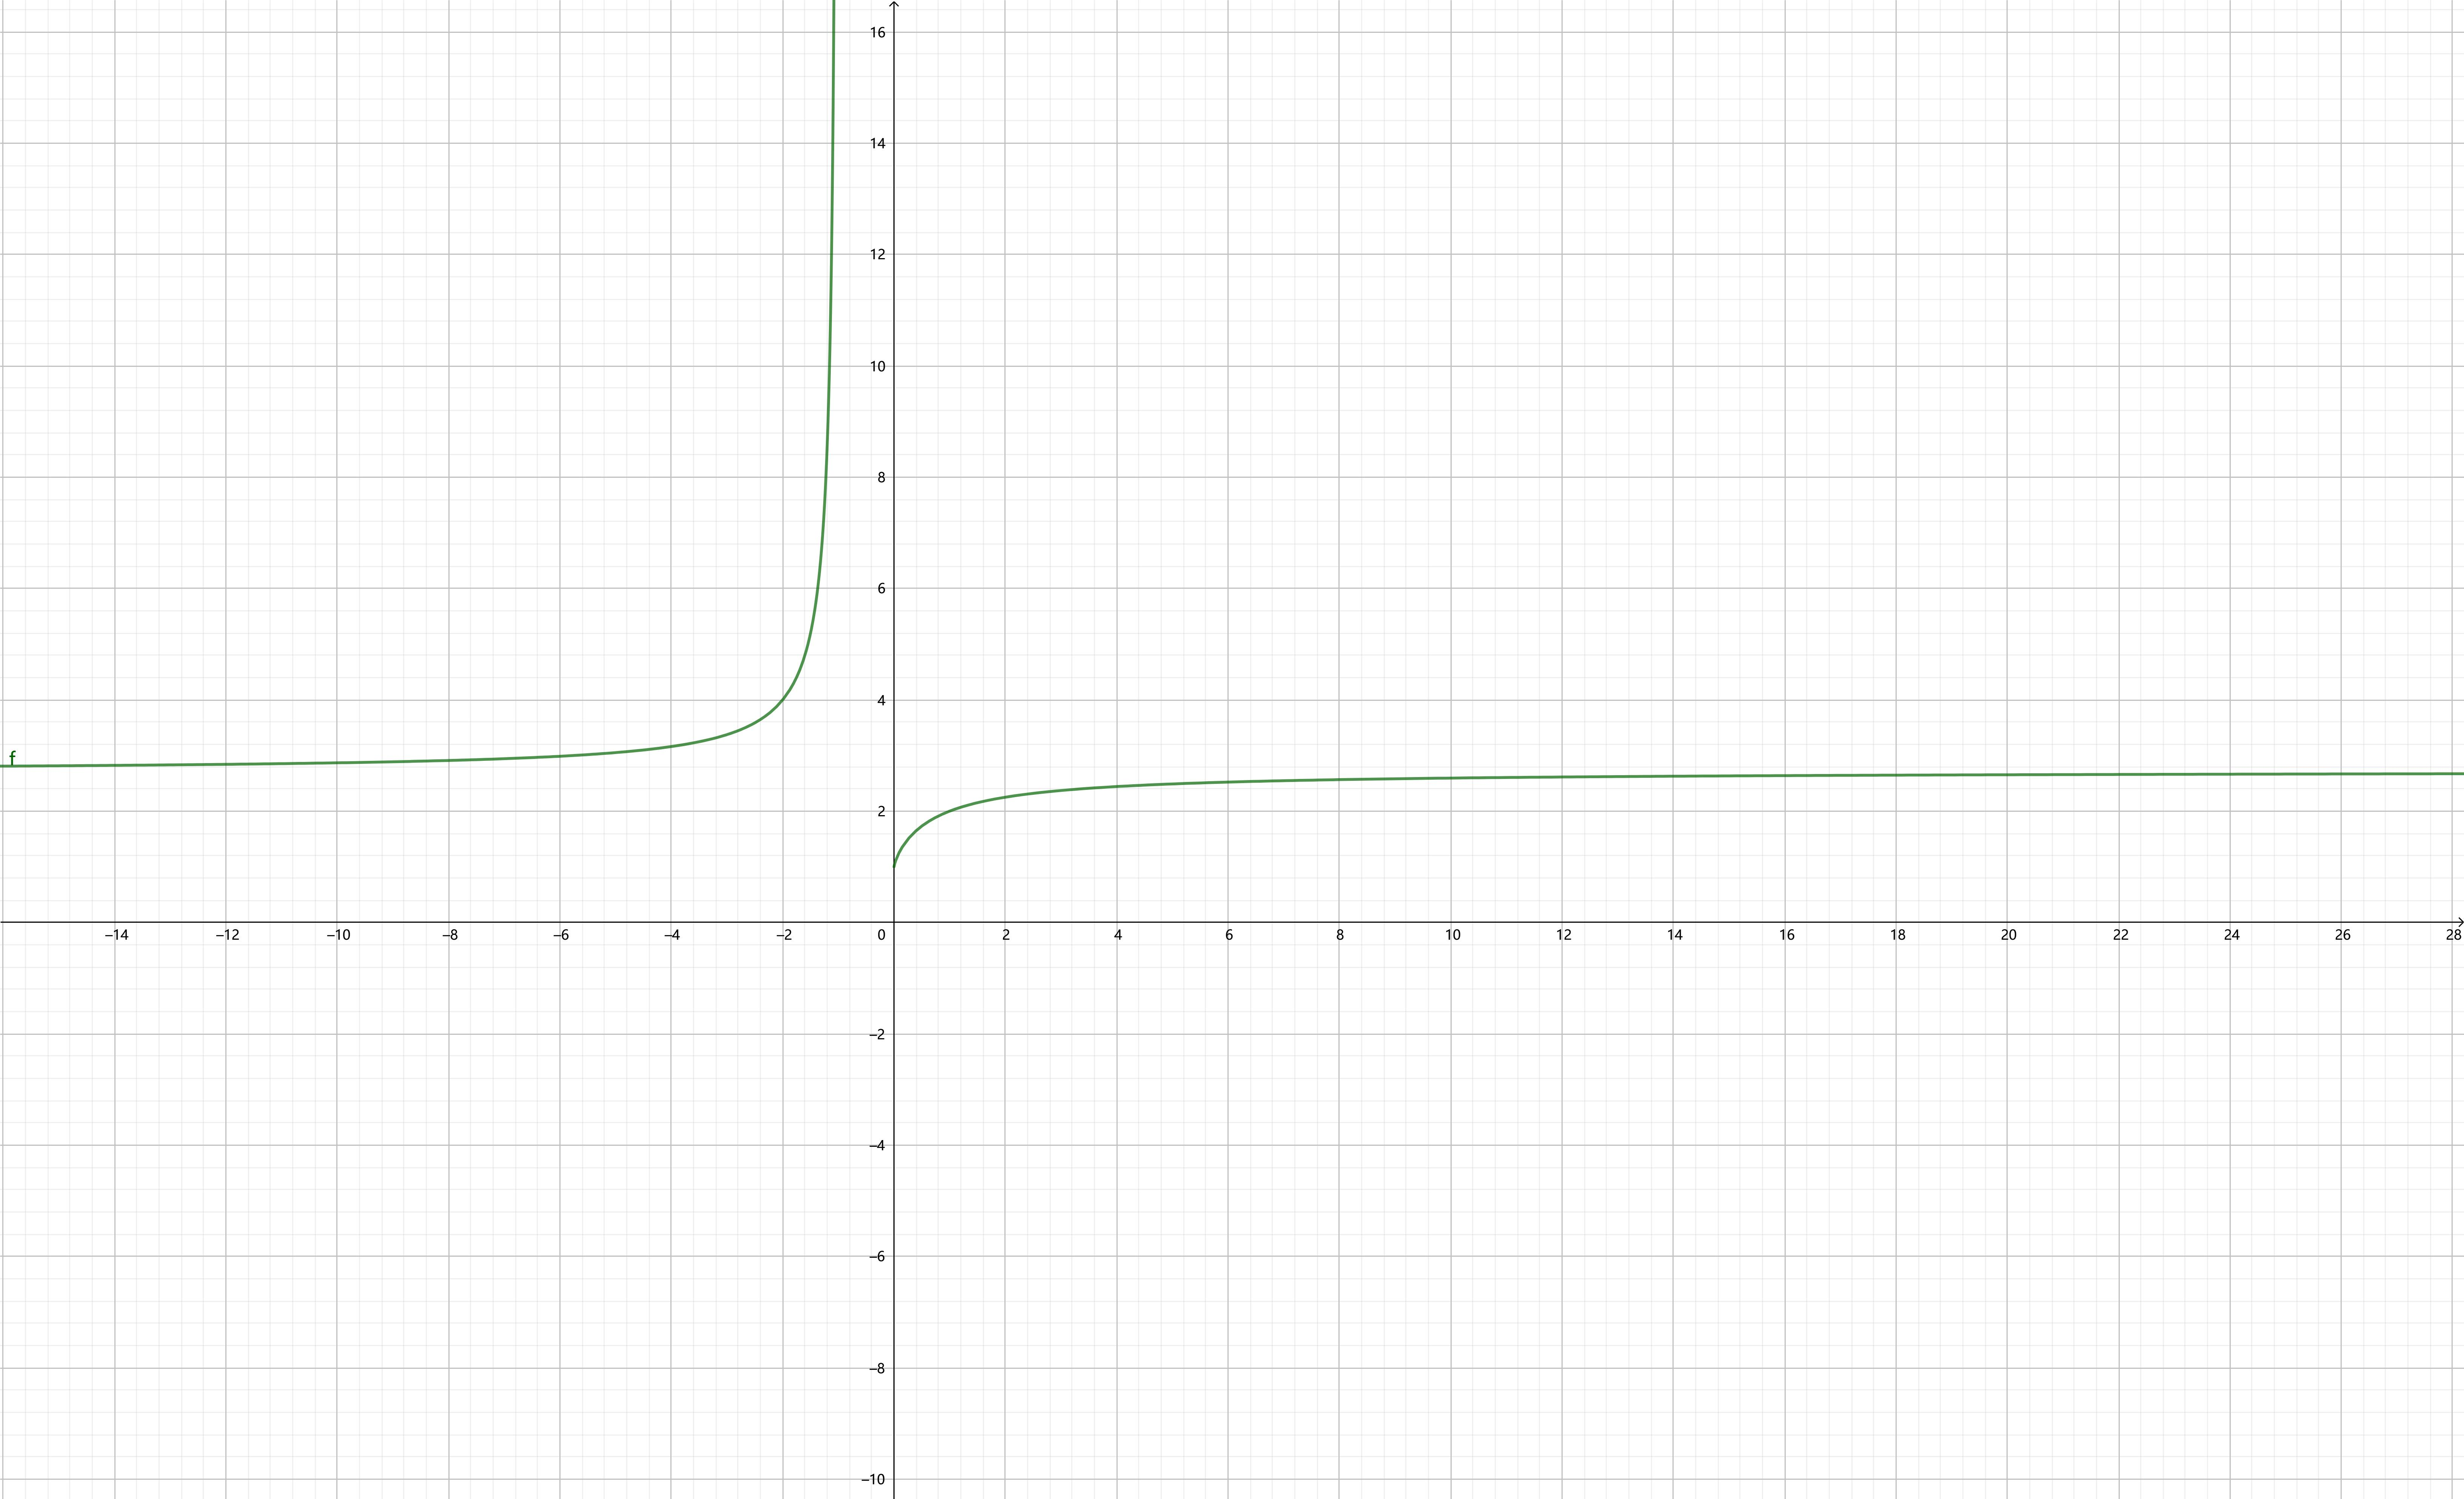
\includegraphics[width=1\linewidth]{res/aaa.jpg}
				\end{figure}
			\end{column}
	\end{columns}
	\end{frame}

    \colortheme{blue!50!black}

	\begin{frame}
		\frametitle{The Precise Definition of a Limit}
		Let $f$ be a function defined on some open interval that contains the number $a$, \alert{except possibly} at $a$ itself. Then we say that the limit if $f(x)$ as $x$ approaches $a$ is $L$, and we write
		\begin{center}
				$\lim\limits_{\textit{x} \to a}f(x) = L$
		\end{center}
		if for \alert{every} number $\varepsilon > 0$, there is a number $\delta > 0$ such that
		\begin{center}
				if\ \ \ $0 < |x - a| < \delta$\ \ \ then\ \ \ $|f(x) - L| < \varepsilon$
		\end{center}
	\end{frame}
	\begin{frame}
		\frametitle{The Precise Definition of a Limit}
		Left-hand limits:
		\begin{center}
				$\lim\limits_{\textit{x} \to a^{-}}f(x) = L$
		\end{center}
		if for \alert{every} number $\varepsilon > 0$, there is a number $\delta > 0$ such that
		\begin{center}
				if\ \ \ $a - \delta < x < a$\ \ \ then\ \ \ $|f(x) - L| < \varepsilon$
		\end{center}
		Right-hand limits:
		\begin{center}
				$\lim\limits_{\textit{x} \to a^{+}}f(x) = L$
		\end{center}
		if for \alert{every} number $\varepsilon > 0$, there is a number $\delta > 0$ such that
		\begin{center}
				if\ \ \ $a < x < a + \delta$\ \ \ then\ \ \ $|f(x) - L| < \varepsilon$
		\end{center}
	\end{frame}
	\begin{frame}
		\frametitle{The Precise Definition of a Limit}
		Infinite limits:\\
		\begin{enumerate}
		\item Let $f$ be a function defined on some open interval that contains the number $a$, \alert{except possibly} at $a$ itself. Then
			\begin{center}
					$\lim\limits_{\textit{x} \to a}f(x) = \infty$
			\end{center}
			means that for \alert{every positive} number $M$, there is a number $\delta > 0$ such that
			\begin{center}
					if\ \ \ $0 < |x - a| < \delta$\ \ \ then\ \ \ $f(x) > M$
			\end{center}
		\item Let $f$ be a function defined on some open interval that contains the number $a$, \alert{except possibly} at $a$ itself. Then
			\begin{center}
					$\lim\limits_{\textit{x} \to a}f(x) = -\infty$
			\end{center}
			means that for \alert{every negative} number $N$, there is a number $\delta > 0$ such that
			\begin{center}
					if\ \ \ $0 < |x - a| < \delta$\ \ \ then\ \ \ $f(x) < N$
			\end{center}
		\end{enumerate}
	\end{frame}
	\begin{frame}
		\frametitle{The Precise Definition of a Limit}
		Limits at Infinity:\\
		\begin{enumerate}
		\item Let $f$ be a function defined on some interval ($a$, $\infty$). Then
			\begin{center}
				$\lim\limits_{\textit{x} \to \infty}f(x) = L$
			\end{center}
			means that for every $\varepsilon > 0$, there is a corresponding number $N$ such that
			\begin{center}
				if\ \ \ $x > N$\ \ \ then\ \ \ $|f(x) - L| < \varepsilon$
			\end{center}
		\item Let $f$ be a function defined on some interval ($-\infty$, $a$). Then
			\begin{center}
				$\lim\limits_{\textit{x} \to -\infty}f(x) = L$
			\end{center}
			means that for every $\varepsilon > 0$, there is a corresponding number $N$ such that
			\begin{center}
				if\ \ \ $x < N$\ \ \ then\ \ \ $|f(x) - L| < \varepsilon$
			\end{center}
	\end{enumerate}
	\end{frame}

    \colortheme{green!30!black}

	\begin{frame}
		\frametitle{Exercise 1}
		Evaluate the following limits\\
		\begin{enumerate}
			\item $\lim\limits_{\textit{x} \to 0}\dfrac{4x^{3}-2x^{2}+x}{2x+3x^{2}}$
			\item $\lim\limits_{\textit{x} \to 0}\dfrac{\dfrac{1}{3+x}-\dfrac{1}{3}}{x}$
			\item $\lim\limits_{\textit{x} \to \infty}(1+\dfrac{1}{x})(2-\dfrac{1}{x^{2}})$
			\item $\lim\limits_{\textit{x} \to 0}\dfrac{-1+\sqrt[n]{x+1}}{x}$

		\end{enumerate}
	\end{frame}
	\colortheme{blue!50!black}
	\begin{frame}
		\frametitle{Exercise 2}
		Evaluate the following limits\\
		\begin{enumerate}
		    \item $\lim\limits_{\textit{x} \to -4}\dfrac{\sqrt{9+x^{2}}-5}{x+4}$
			\item $\lim\limits_{\textit{\alert{h}} \to 0}\dfrac{(x+h)^{3}-x^{3}}{h}$(What if $\lim\limits_{\textit{\alert{h}} \to 0}\dfrac{(x+h)^{n}-x^{n}}{h}$?)
			\item $\lim\limits_{\textit{x} \to 0}\dfrac{\sin{\omega x}}{x}$
			\item $\lim\limits_{\textit{x} \to \infty}(1-\dfrac{1}{x})^{kx}$\ \ \ ($k$ is a positive integer)
			\item $\lim\limits_{\textit{x} \to \dfrac{\pi}{2}}(\sin{x})^{\tan{x}}$
		\end{enumerate}
	\end{frame}
	\colortheme{green!30!black}
	\begin{frame}
		\frametitle{Conclusions}
		Some methods to calculate the limits:
		\begin{enumerate}
			\item Use those limit laws directly
			\item Exchange the order of functions and limit symbols based on the continuity of composite function. (Will be mentioned later)
			\item Do factorization, denominator rationalization or numerator rationalization.
			\item If a factor approaching zero is find in the denominator, try to eliminate it.
			\item Translate the formula into the form of "two important limits"
			\item \alert{The method to solve those formulas having the form of $u(x)^{v(x)}$ will be discussed at a deeper level after the differentiation and l'Hôpital's rule are taught.}
		\end{enumerate}
	\end{frame}
	\begin{frame}{Exercise Answer 1}
	    \begin{enumerate}

			\item $\lim\limits_{\textit{x} \to 0}\dfrac{4x^{3}-2x^{2}+x}{2x+3x^{2}}=\lim\limits_{\textit{x} \to 0}\dfrac{4x^{2}-2x+1}{2+3x}$=0.5
			\item $\lim\limits_{\textit{x} \to 0}\dfrac{\dfrac{1}{3+x}-\dfrac{1}{3}}{x}=\lim\limits_{\textit{x} \to 0}\dfrac{3-3-x}{3x(3+x)}=\lim\limits_{\textit{x} \to 0}\dfrac{-1}{3(3+x)}=-\dfrac{1}{9}$
			\item $\lim\limits_{\textit{x} \to \infty}(1+\dfrac{1}{x})(2-\dfrac{1}{x^{2}})=\lim\limits_{\textit{x} \to \infty}(1+\dfrac{1}{x})\cdot\lim\limits_{\textit{x} \to \infty}(2-\dfrac{1}{x^{2}})=1\cdot2=2$
			\item Let $t^{n}-1:=x$, $\lim\limits_{\textit{x} \to 0}\dfrac{-1+\sqrt[n]{x+1}}{x}=\lim\limits_{\textit{t} \to 1}\dfrac{t-1}{t^{n}-1}=\lim\limits_{\textit{t} \to 1}\dfrac{1}{1+t+t^2+\cdots+t^{n-1}}=\dfrac{1}{n}$
		\end{enumerate}
	\end{frame}
	\colortheme{blue!50!black}
	\begin{frame}{Exercise Answer 2}
	    \small
	    \begin{enumerate}
		    \item $\lim\limits_{\textit{x} \to -4}\dfrac{\sqrt{9+x^{2}}-5}{x+4}=\lim\limits_{\textit{x} \to -4}\dfrac{x-4}{\sqrt{9+x^{2}}+5}=-\dfrac{4}{5}$
			\item $\lim\limits_{\textit{\alert{h}} \to 0}\dfrac{(x+h)^{n}-x^{n}}{h}=\lim\limits_{\textit{\alert{h}} \to 0}nx^{n-1}+h\cdot(\cdots)=nx^{n-1}$
			\item $\lim\limits_{\textit{x} \to 0}\dfrac{\sin{\omega x}}{x}=\omega\cdot\lim\limits_{\textit{x} \to 0}\dfrac{\sin{\omega x}}{\omega x}=\omega$
			\item $\lim\limits_{\textit{x} \to \infty}(1-\dfrac{1}{x})^{kx}=\lim\limits_{\textit{x} \to \infty}(1+\dfrac{1}{-x})^{(-x)(-k)}=e^{-k}$
			\item $\lim\limits_{\textit{x} \to \dfrac{\pi}{2}}(\sin{x})^{\tan{x}}=\lim\limits_{\textit{x} \to \dfrac{\pi}{2}}(1+(\sin{x}-1))^{\dfrac{1}{\sin{x}-1}\cdot(\sin{x}-1)\tan{x}}=e^{\lim\limits_{\textit{x} \to \dfrac{\pi}{2}}(\sin{x}-1)\tan{x}}=e^{\lim\limits_{\textit{x} \to \dfrac{\pi}{2}}\dfrac{(\sin{x}-1)\sin{x}}{\sqrt{1-\sin^2x}}}=e^{-\lim\limits_{\textit{x} \to \dfrac{\pi}{2}}\dfrac{\sqrt{1-\sin{x}}\sin{x}}{\sqrt{1+\sin x}}}=e^0=1$
		\end{enumerate}
		\normalsize
	\end{frame}
	\colortheme{green!30!black}




	\begin{frame}{References}
	    \frametitle{References}
		[1] Huang, Yucheng. VV156\_RC2.pdf. 2021.\\
		\bigskip
		[2] Cai, Runze. Chapter01.pdf. 2021.\\
		\bigskip
		[3] Department of mathematics, Tongji University. Advanced Mathematics (7th Edition). 2014.\\
		\bigskip
		[4] James Stewart. Calculus (7th Edition). 2014.\\
		\bigskip
		[5] Department of mathematics, Tongji University. Learning Guidance of Advanced Mathematics (7th Edition). 2014.\\
		\bigskip
		[6]Zhou,Yishen.RC2. 2022.
	\end{frame}